\section{Funktion der Bleibatterie}

Die Technik der Bleibatterien hat eine lange Geschichte welche bis in die Mitte des 19. Jahrhunderts zurückreicht. Diese sind heute in der Automobilindustrie eine schlechte und veraltete Alternative verglichen mit den modernen Lithium-Ionen-Akkumulatoren (siehe Kapitel \ref{kap_liion}). Zu dieser Zeit waren Bleibatterien jedoch die einzig sinnvolle Lösung Energie für den Eigengebrauch zu speichern. In diesem Kapitel soll die Grundfunktion einer Bleibatterie und die Lade-/Entladekurve erläutert werden.

\paragraph{Grundfunktion}
Grundsätzlich kommt die Bezeichnung Bleiakkumulator davon, dass beide Elektroden aus Blei, bzw. die positive Elektrode aus Bleidioxid (PbO$_2$) und die negative aus blankem Blei (Pb), besteht. Das Elektrolyt, was sich zwischen den Platten befindet, besteht aus Schwefelsäure (H$_2$SO$_4$). Im geladenen Zustand kann nun eine externe leitende Verbindung zwischen den beiden Elektroden gelegt werden. Dadurch zersetzt sich die positive Elektrode unter Elektronenabgabe, während die negative Elektrode Elektronen aufnimmt. Somit findet ein Ionenaustausch statt. Durch diesen Prozess wird der Akkumulator entladen und beide Elektroden bestehen nun aus Bleisulfat (PbSO$_4$). Der Ladeprozess funktioniert umgekehrt zum Entladeprozess. Durch Anlegen einer Spannung werden die Ionen wieder vom Minus- zum Plus-Pol transportiert. Auf weitere chemische Beschreibungen wird an dieser Stelle verzichtet. Der Lade- und Entladevorgang ist in Figur \ref{fig:pb_akku} ersichtlich \cite{pb_akku_funktion}:

\begin{figure}[h!]
	\centering
		\includegraphics[width=0.75\textwidth]{images/pb_akku.PNG}
	\caption{Lade-/Entladevorgang Blei-Akkumulator \cite{pb_akku_ent_lade}}
	\label{fig:pb_akku}
\end{figure}

\newpage

\paragraph{Lade-/Entladekurve}
Die Lade-/Entladekurve ist abhängig vom jeweiligen Akkumulatortyp. So auch die Bleibatterie, welche in Figur \ref{fig:pb_akku_kurve} für ein einzelnes Modul ersichtlich ist:

\begin{figure}[h!]
	\centering
		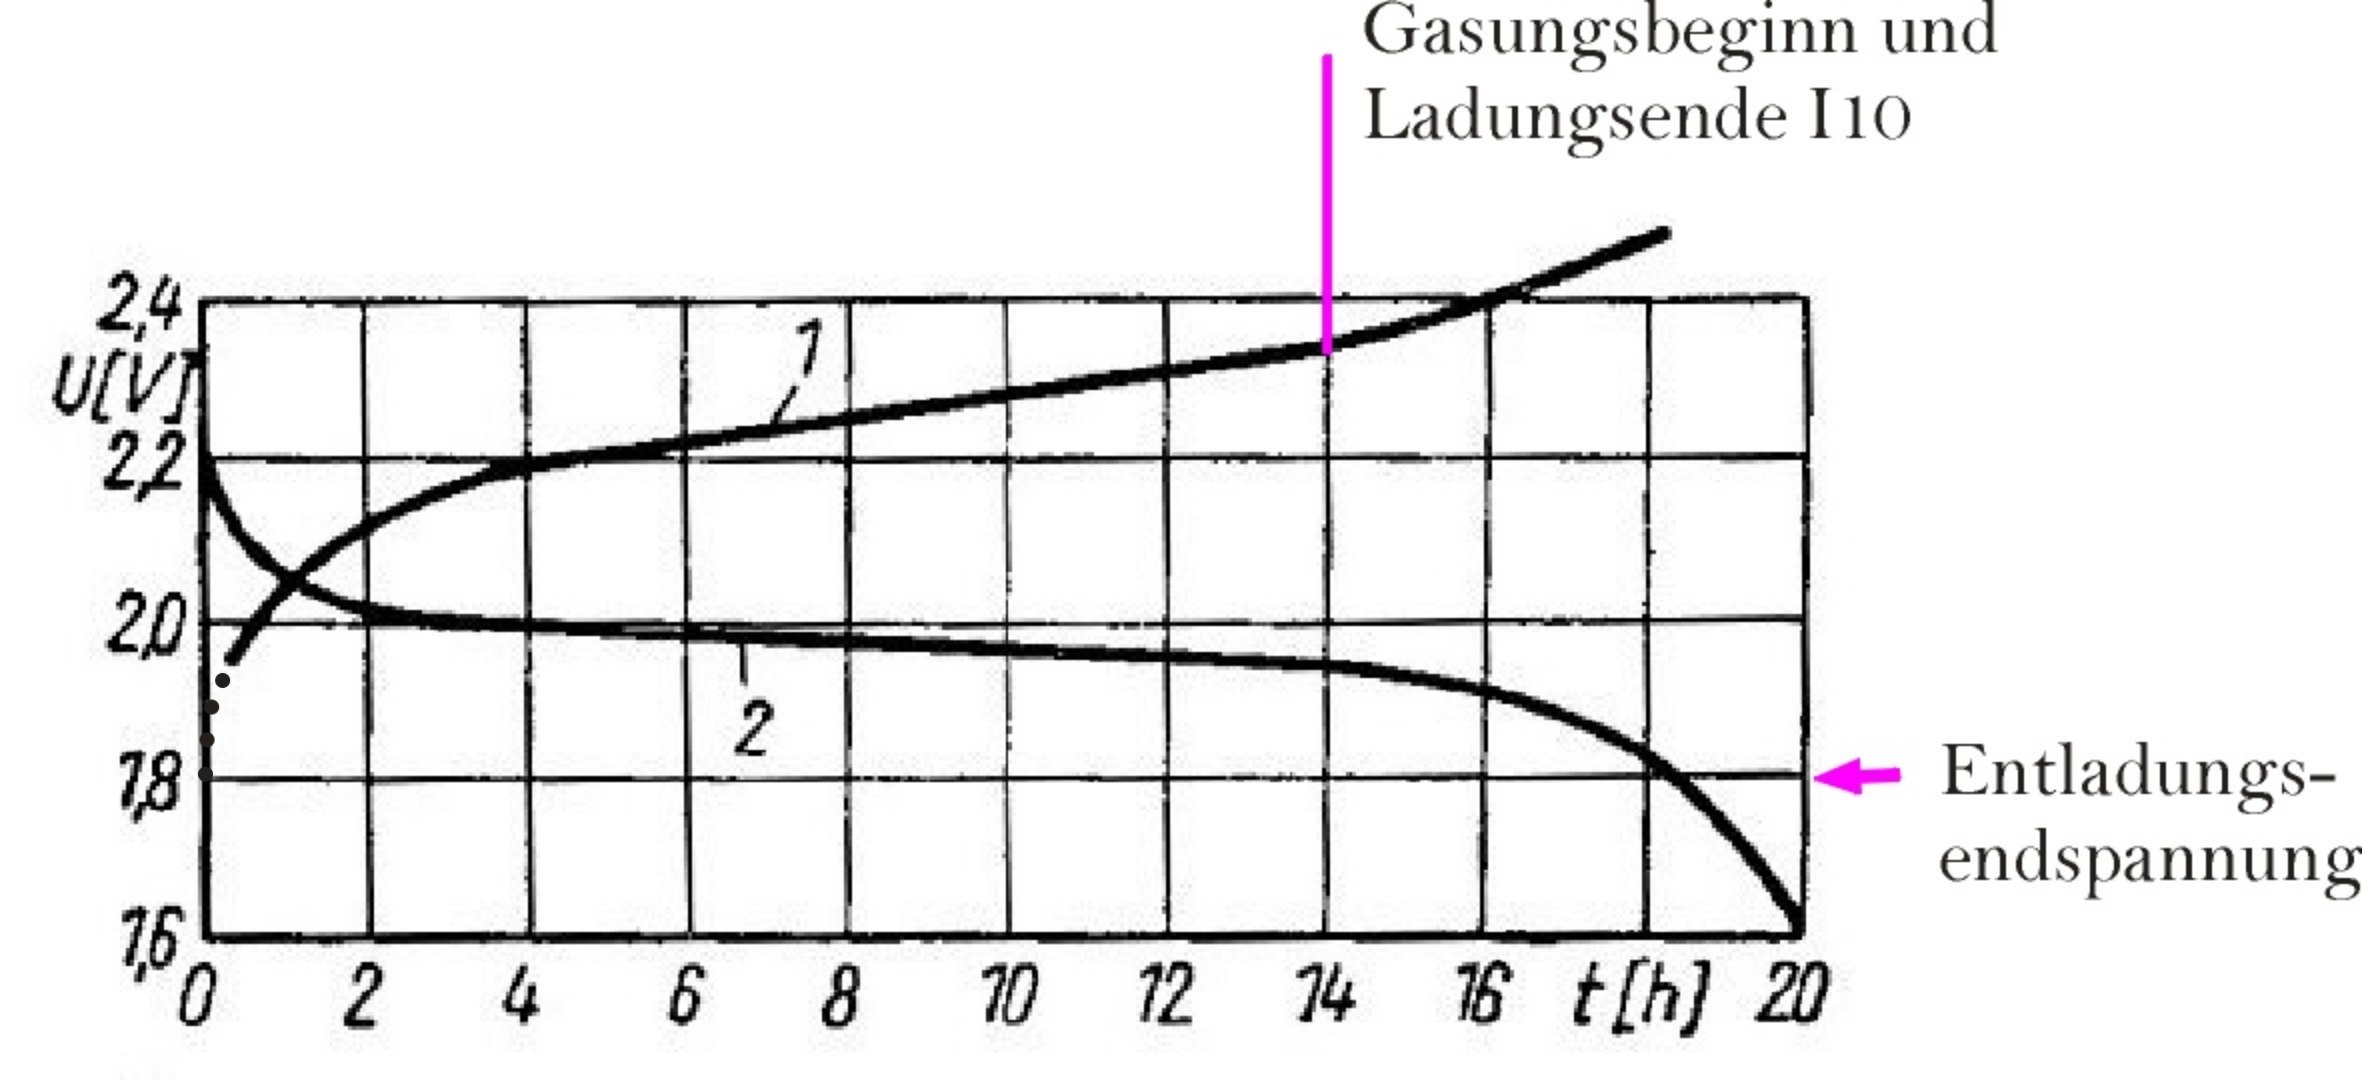
\includegraphics[width=0.8\textwidth]{images/pb_akku_kurve.jpg}
	\caption{Lade-/Entladekurve Blei-Akkumulator \cite{pb_akku_kurve}}
	\label{fig:pb_akku_kurve}
\end{figure}

Aus der obigen Figur ist ersichtlich, dass die Kurve im Zeitraum von 4 bis 14 Stunden einen konstante Anstieg im Ladevorgang oder Abstieg im Entladevorgang besitzt. Was unbedingt beachtet werden muss ist, dass ein einzelnes Bleimodul nicht unter $1.8$ V entladen oder über $2.3$ V geladen werden sollte. Dies könnte sonst zu einer Zerstörung des Moduls führen.

\newpage